\begin{section}{N-body Simulation of Dark Matter Density Fields}
  \label{sec:simulation}
    We run 139 simulations with a box size of 300 $h^{-1}$Mpc, resolution of $1024^3$ cells and $512^3$ particles, using the cosmological simulation code CubeP3M(CITA Computing 2008?).The initial condition is given by reading CMBFAST transfer function and then evolving the power linearly to $z=100$. Then Zel'dovich approximation is used to calculate the displacement field and velocity field, which are assigned to the particles. The cosmological parameters used are $\Omega_M=0.32$, $\Omega_{\Lambda}=0.679$, $h=0.67$, $\sigma_8=0.83$, and $n_s=0.96$. And we use different seeds to produce the initial conditions for different simulations so that those simulations are indipendent to each other. Then the initial densities are evolved up to $z=0$. Projection of one of those density fields is plotted in Fig. \ref{fig:simandrec} (a), in which the magnitude is the average of number of particles per cell over the dimension perpendicular to the paper.
\begin{figure*}
\centering
 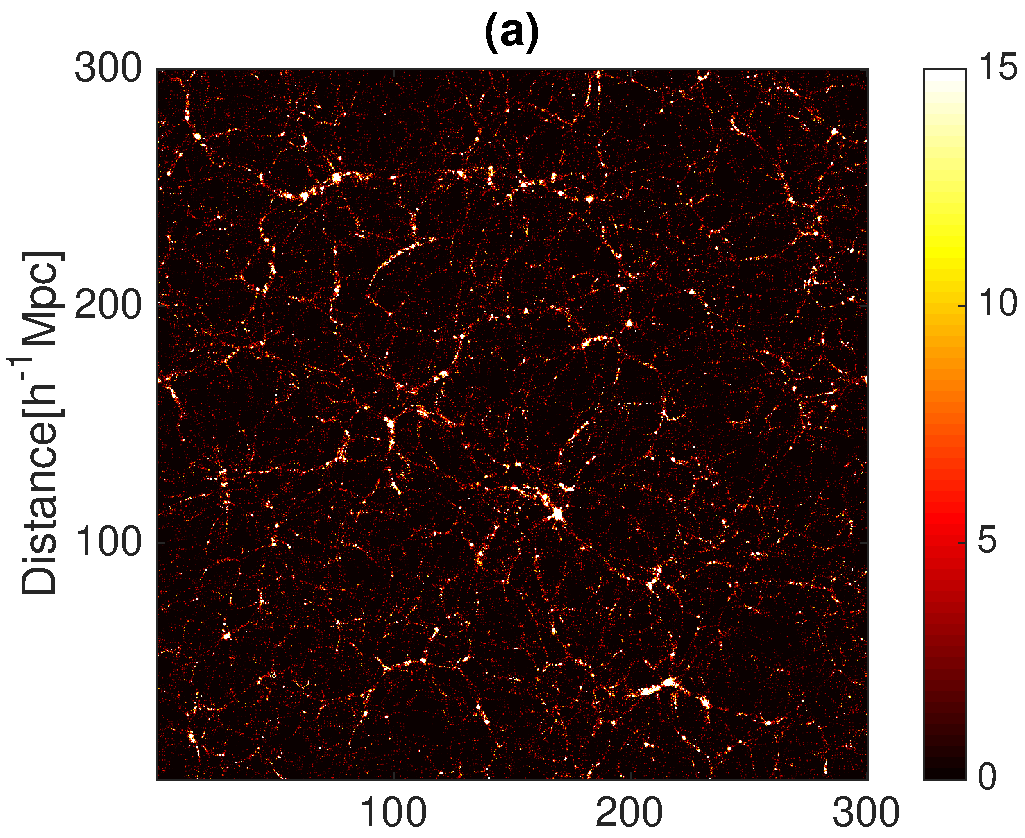
\includegraphics[width=0.8\textwidth]{simulation-crop.pdf}
 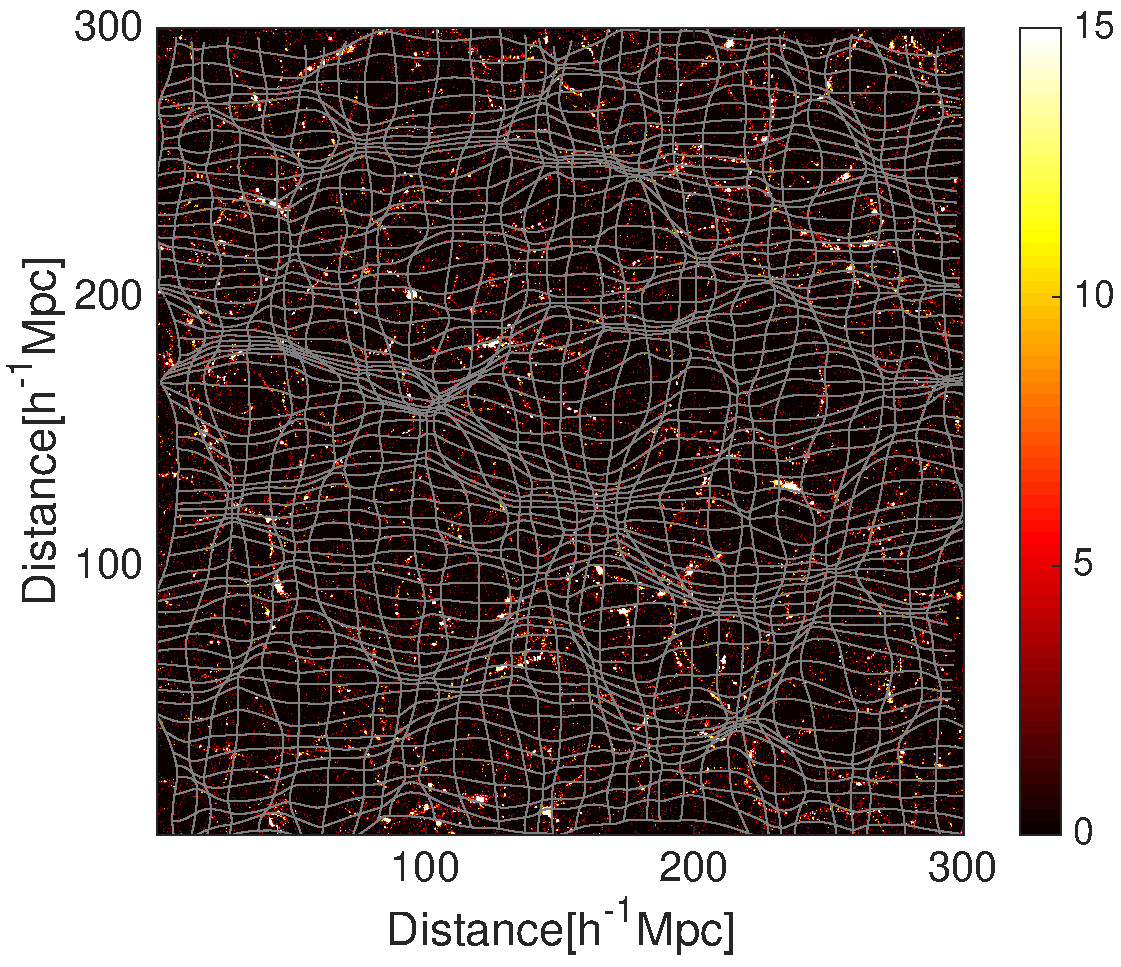
\includegraphics[width=0.8\textwidth]{reconstruction-crop.pdf}
%\begin{tabular}{cc}
% \begin{minipage}[t]{0.48\textwidth}
%  \centering
%  \includegraphics[width=12cm]{simulation.eps}
%  \label{fig:simulation}
% \end{minipage}\\
% \begin{minipage}[t]{0.48\textwidth}
% \centering
%  \includegraphics[width=7cm]{reconstruction.eps}
%  \label{fig:reconstruction}
% \end{minipage}
%\end{tabular}
 \label{fig:simandrec}
   \caption{(a) Map of a randomly selected density field from 139 N-body simulations, with a 300 $h^{-1}$Mpc width box and $1024^3$ pixels. It's the projection along the axis perpendicular to the paper, and the magnitude is the average of number of particles per cell.(b) The density field and the deformed grids of a random selected layer of the selected density field in (a).}
\end{figure*}

\end{section}

